\section{Requirement specification}
In this section a package diagram will give an overview of the different diagrams included and where they belong. A Use case diagram showing the different use cases that where extracted from the project description found on page \pageref{sc:problemdescription}. The section also contains use case descriptions and a list of requirements.
\subsection{Description}

\noindent\fbox{
	\parbox{\textwidth}{
		\textbf{2.} Write a requirement specification with functional and non-functional requirements especially with focus on performance like throughput and latency. The functional requirements can be	described in terms of use cases.
	}
}\citepawesome{Bjerge2017}{1}


\subsection{Analyzing the Problem}
To make a Domain Model we start by a analysis of the description on page \pageref{sc:problemdescription}. Here we find the following nouns in the text and then they can be used later to get a good cobbling between problem and models.

\textbf{This could be removed if it does not make sense}



\subsection{Model Organization}
To manage the complete model and sub-models of the full system, the package diagram\citepawesome{Friedenthal2014}{103} will be used. A package diagram is a system organization model of SysML standards. In this project the package diagram will be used to formulate and verify which diagrams and models are used as a methodology to describe the system of interest. Another effect the package diagram have on this project, is the organization structure it brings.\\

Multiple package diagrams are used to explain dependencies of components and sub-systems in a complex system. Since this project is of a smaller scale, only a single package diagram is needed. However this 

\subsection{Operation}
\blindtext

%==================== Fully Dressed Use Cases ====================

\subsubsection{Use Case Diagram} \label{sec:usecasediagrams}

\blindtext
%For alle Use Cases hvor brugeren navigerer i undermenuer af hovedmenuen, gælder det, at brugeren har mulighed for at gå et skridt tilbage ved at trykke på en ”tilbage knap”. Fremover ved benævningen ”Systemet er operationelt” menes, at systemet er tilsluttet strømforsyning og at alt fungerer samt at systemet er tilsluttet ethernet.

\begin{figure}[!h]
	\centering
	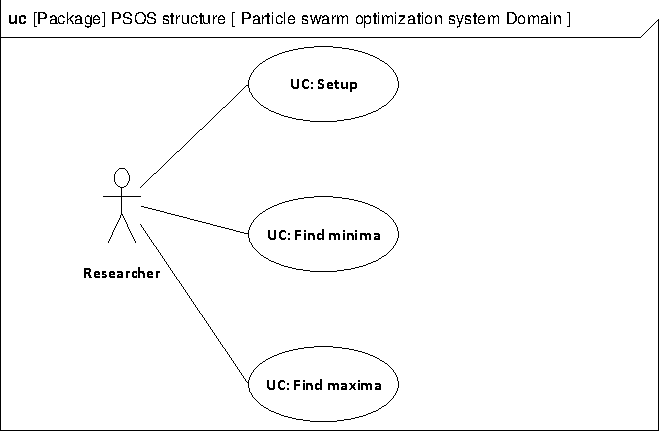
\includegraphics[width=0.8\linewidth]{diagram/uc_particle_swarm_optimization_system.pdf}
	\caption{Use Case Diagram of Particle Swarm Optimization}
	\label{fig:ucdiagram}
\end{figure}


%-------------------- UC1 --------------------
\begin{table}[h]
\begin{tabularx}{\textwidth}{| >{\raggedright\arraybackslash}p{3.3 cm} | >{\raggedright\arraybackslash}X |} \hline

\textbf{Name:} 						& UC1: Start\\ \hline
\textbf{Goal:}						&  \\ \hline
\textbf{Initering:}					&  \\ \hline
\textbf{Actor:} 					& User (primær) \\ \hline
\textbf{Reference:} 					& UC10: Monitorering, UC11: Regulering \\ \hline
\textbf{Number of simultaneous occurrences:} & Én \\ \hline
\textbf{Pre-condition:} 				& \\ \hline
\textbf{Result:}					&  \\ \hline
\textbf{Main scenario:}				& 

\begin{packed_enum}
\item allaa
\item allala
\item alllaa
	\begin{packed_item}\itemsep1pt \parskip0pt \parsep0pt
	\item {[}Ext 3.a : User does not press "Regulation".{]}
	\end{packed_item}
\item Systemet aktiverer UC11: Regulering.
\item UC1 afsluttes.
\end{packed_enum} \\ \hline
\textbf{extensions:}				&  
\textbf{{[}Ext 3.a :User selects only monitoring.{]}}
	\begin{packed_enum}\itemsep1pt \parskip0pt \parsep0pt
	\item The system continues at point. 5 in the main scenario.
	\end{packed_enum}
\\ \hline
\end{tabularx}
\caption{UC1: Start}
\label{tbl:uc1}
\end{table}
%-------------------- UC2 --------------------
\begin{table}[h]
	\begin{tabularx}{\textwidth}{| >{\raggedright\arraybackslash}p{3.3 cm} | >{\raggedright\arraybackslash}X |} \hline
		
		\textbf{Name:} 						& UC2: Find minima\\ \hline
		\textbf{Goal:}						& Find the minima of a function \\ \hline
		\textbf{Initering:}					& Researcher \\ \hline
		\textbf{Actor:} 					& Researcher (primary) \\ \hline
		\textbf{Reference:} 				& UC1: Setup \\ \hline
		\textbf{Number of simultaneous occurrences:} & One \\ \hline
		\textbf{Pre-condition:} 				& UC1 has been done \\ \hline
		\textbf{Result:}					& Found the minima of a function \\ \hline
		\textbf{Main scenario:}				& 
		
		\begin{packed_enum}
			\item allaa
			\item allala
			\item alllaa
			\begin{packed_item}\itemsep1pt \parskip0pt \parsep0pt
				\item {[}Ext 3.a : User does not press "Regulation".{]}
			\end{packed_item}
			\item Systemet aktiverer UC11: Regulering.
			\item UC1 afsluttes.
		\end{packed_enum} \\ \hline
		\textbf{extensions:}				&  
		\textbf{{[}Ext 3.a :User selects only monitoring.{]}}
		\begin{packed_enum}\itemsep1pt \parskip0pt \parsep0pt
			\item The system continues at point. 5 in the main scenario.
		\end{packed_enum}
		\\ \hline
	\end{tabularx}
\caption{UC2: Start}
\label{tbl:uc2}
\end{table}
%-------------------- UC3 --------------------
\begin{table}[h]
\begin{tabularx}{\textwidth}{| >{\raggedright\arraybackslash}p{3.3 cm} | >{\raggedright\arraybackslash}X |} \hline

\textbf{Navn:} 						& UC1: Start\\ \hline
\textbf{Mål:}						& At starte systemet helt eller delvist. \\ \hline
\textbf{Initering:}					& Bruger \\ \hline
\textbf{Aktører:} 					& Bruger (primær) \\ \hline
\textbf{Reference:} 					& UC10: Monitorering, UC11: Regulering \\ \hline
\textbf{Antal samtidige forekomster:} & Én \\ \hline
\textbf{Forudsætning:} 				& Systemet er stoppet helt, er operationelt og viser hovedmenuen.\\ \hline
\textbf{Resultat:}					& UC10: Monitorering og evt. UC11: Regulering er startet, systemet viser Hovedmenuen. \\ \hline
\textbf{Hovedscenarie:}				& 

\begin{packed_enum}
\item Bruger trykker på "Monitorering". 
\item System aktiverer UC10: Monitorering. 
\item Bruger trykker på "Regulering". 
	\begin{packed_item}\itemsep1pt \parskip0pt \parsep0pt
	\item {[}Ext 3.a : Bruger trykker ikke "Regulering".{]}
	\end{packed_item}
\item Systemet aktiverer UC11: Regulering.
\item UC1 afsluttes.
\end{packed_enum} \\ \hline
\textbf{Udvidelser:}				&  
\textbf{{[}Ext 3.a : Bruger vælger kun monitorering.{]}}
	\begin{packed_enum}\itemsep1pt \parskip0pt \parsep0pt
	\item Systemet fortsætter ved pkt. 5 i hovedscenariet.
	\end{packed_enum}
\\ \hline
\end{tabularx}
\caption{UC3: Start}
\label{tbl:uc3}
\end{table}

\subsubsection{Requirements}
